% This is samplepaper.tex, a sample chapter demonstrating the
% LLNCS macro package for Springer Computer Science proceedings;
% Version 2.20 of 2017/10/04
%
\documentclass[runningheads]{llncs}

\usepackage{graphicx}   % Images
\usepackage{tabularx}   % Tables
\newcolumntype{C}{>{\centering\arraybackslash}X} % Table uses all width and it's centered
\usepackage{hyperref}
\hypersetup{
    colorlinks = true,
    linkcolor = blue,
    filecolor = blue,
    citecolor = black,      
    urlcolor = black,
}

% If you use the hyperref package, please uncomment the following line
% to display URLs in blue roman font according to Springer's eBook style:
% \renewcommand\UrlFont{\color{blue}\rmfamily}

\begin{document}
% Title
\title{Solver of Tricky Triple Puzzles Based on Constraint Programming}
% Abbreviated Title
\titlerunning{Tricky Triple Solver}

% Authors
\author{
    \begin{tabular}{l r}
        \email{up201303828@fe.up.pt} & Ângelo Daniel Pereira Mendes Moura \\
        \email{up201806528@fe.up.pt} & Clara Alves Martins \\
    \end{tabular}
}
\authorrunning{Ângelo Moura \and Clara Martins}

% Institutes
\institute{Faculty of Engineering of the University of Porto \\
\url{https://www.fe.up.pt} \\
\centering

\includegraphics[scale=0.2]{img/FEUPlogo.png}
}

\maketitle              % typeset the header of the contribution

\begin{center}
    \large{\textbf{Logic Programming}} \\
    \normalsize{3MIEIC06 - Tricky Triple 2}
\end{center}

\begin{center}
    \large{\textbf{\today}} % Date for the report
\end{center}

\begin{abstract}
In this article, we show how to use constraint programming to solve Tricky Triple Puzzles.
We present a consistent method to analyze these puzzles and to obtain a solution to them.

\keywords{tricky-triple \and prolog \and clpfd \and constraint-programming}
\end{abstract}

% Contents
\section{Introduction}
This project consists of building a program, in Logic Programming with Restrictions,
    for solving a combinatorial decision.
The problems studied are Tricky Triple Puzzles, which are grid puzzles. 
To do so, we will analyze these problems and proceed to implement our solver using SICStus Prolog.
Afterward, we will be discussing the performance results obtained.
This article has the following structure:
\begin{itemize}
    \item \textbf{Problem Description}: tricky triple puzzle detailed description
    \item \textbf{Approach}: problem modulation
        \begin{itemize}
            \item \textbf{Decision Variables}: decision variables' meaning and domain
            \item \textbf{Constraints}: problem constraints' description
        \end{itemize}
    \item \textbf{Solution Presentation}: explanation for the predicates that provide a user interface
    \item \textbf{Experiments and Results}: results from all the tests
        \begin{itemize}
            \item \textbf{Search Strategies}: result's analysis from different search strategies
            \item \textbf{Dimensional Analysis}: result's analysis from different puzzle's dimensions
        \end{itemize}
    \item \textbf{Conclusions and Future Work}: conclusions withdraw and limitations of this project
    \item \textbf{References}: books, web pages, and articles used
    \item \textbf{Annex}: result tables and other extras
\end{itemize}

\section{Problem Description}
The Tricky Triple puzzles are a type of grid puzzle.
The goal of the puzzle is to fill each of the grid’s white cells with one of 3 symbols,
a square, a circle, or a triangle.
The only rule is that each group of 3 adjacent white cells
    (horizontally, vertically, or diagonally) must contain exactly 2 of one of the symbols.
So, each group of 3 white cells will have 2 of 3 symbols.
Each puzzle given has a unique solution.

\begin{figure} [h]
    \centering
    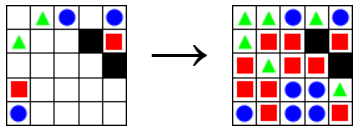
\includegraphics[scale=0.7]{img/tricky-triple.png}
    \caption{Example of Tricky Triple Puzzles, before and after solving it} \label{fig1}
\end{figure}

\section{Approach}
Throughout the development of this project, we used a Constraint Logic Programming approach.
Our grid is a list of lists, where each element is a number indicating the symbol placed on that cell.
Each one of these numbers represents a different symbol.
The number 0 represents a black cell, which cannot be generated by the solver.
The number 1 represents a green triangle,
    while the number 2 represents a red square and the number 3 a blue circle.

\subsection{Decision Variables}
All tricky triple puzzles take the form of an NxN square grid divided by cells.
The grid is represented internally by a list of lists forming a square matrix.

The grid cells can either be black, a cell that the program can't fill, or, more commonly, white.

All the white cells need to be either a triangle (represented by 1), a square (represented by 2),
    or a circle (represented by 3) to reach the puzzle solution.

The Decision Variables are all the elements of the list of lists, meaning all the puzzle cells.
Their domain is {0, 1, 2, 3}. However, being the representative of a black cell,
    the zero is not considered a valid value to fill an empty cell,
    since that would transform a white cell into a black cell.

\subsection{Constraints}
The restrictions implemented in our solver are faithful to the ones from the puzzle rules.

\textbf{Each cell must contain a symbol} \\
In the puzzle solution, all the cells have to be assigned.

\textbf{No black cells can be assigned} \\
In every white cell, we need to put a square, a triangle, or a circle.
Meaning we can't put a black cell on a white cell.

\textbf{Each group of 3 adjacent white cells (horizontally, vertically, or diagonally)
    must contain exactly 2 of one of the symbols} \\
Consider a group of three adjacent, horizontally, vertically, or diagonally, white cells.
In this group, two of the cells have the same symbol, and the last cell must have a different one.

\section{Solution Presentation}
To present the solution, we use two predicates from the file \textit{display.pl}.
\begin{itemize}
    \item The predicate \verb|display_grid/2| displays the grid in a human-friendly way so that
        the user can identify the cells and the grid's symbols.
    \item The predicate \verb|get_readable_symbol/2| translates the grid elements' internal representation
        into more readable symbols for those to be displayed to the user.
\end{itemize}

\begin{figure} [h]
    \centering
    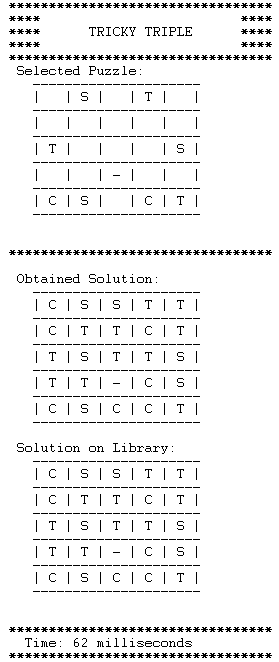
\includegraphics[scale=0.6]{img/puzzle_solving.png}
    \caption{Output Example for a Puzzle Solution} \label{fig2}
\end{figure}

\section{Experiments and Results}
The tests performed on this solver aren't as exhaustive as we could have hoped since
    we could only use the pre-generated puzzles, and there weren't that many of them.
However, we can still draw some conclusions from the times measured when solving these puzzles.

\subsection{Search Strategies}
To compensate for our lack of different puzzles, we did extensive tests with the predefined ones.
After that, we grouped the tests by the puzzle's dimension and the labeling options used in that solution.

From all the collected information, we can withdraw some conclusions:
\begin{itemize}
    \item A small board with bad labeling options can take more time to solve
            than a bigger one with good labeling options.
    \item When introducing some partially solved boards, the solver would be consistently faster.
    \item The solver's execution time increases with the increase in the grid's dimensions.
\end{itemize}

The graph below illustrates the obtained results.
Table \ref{tab1} contains the average values for each dimension and labeling option.

\begin{figure} [h]
    \centering
    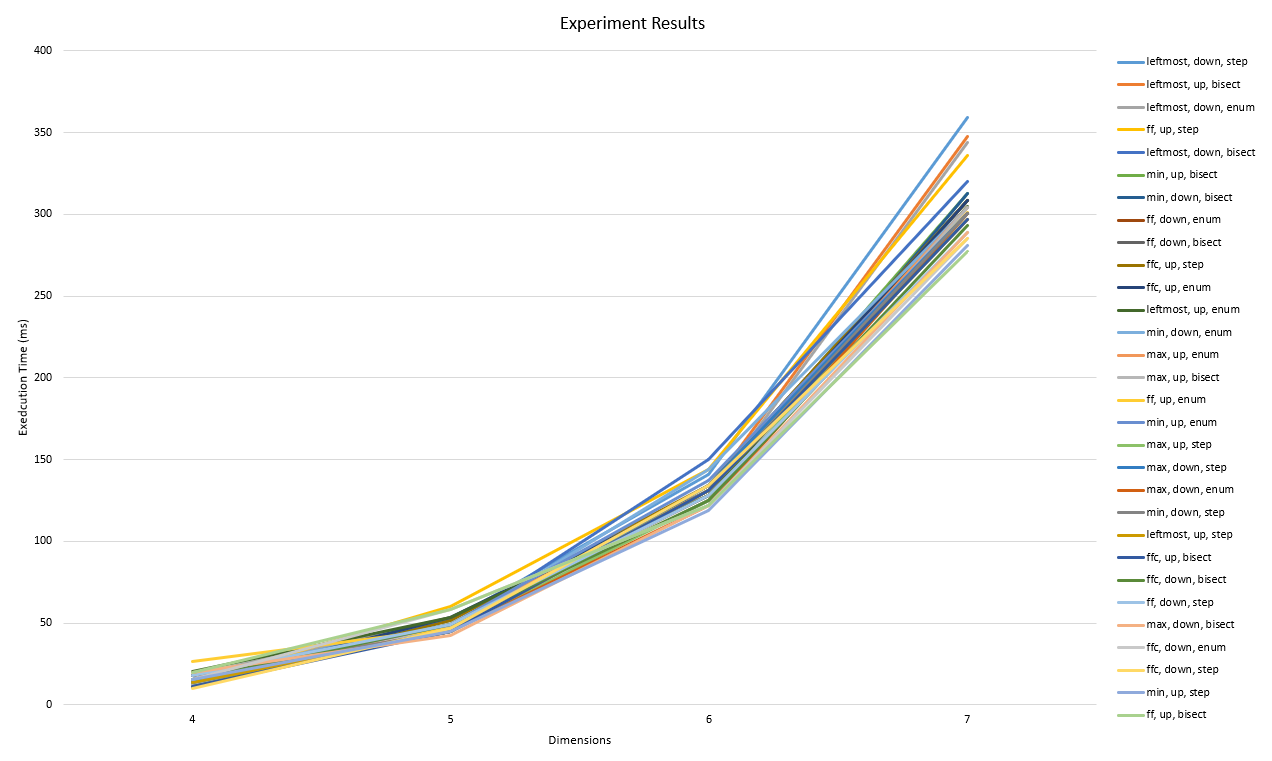
\includegraphics[width=\textwidth]{img/execution_times.png}
    \caption{Experiment Results} \label{fig3}
\end{figure}
Analyzing Figure \ref{fig3}, we can conclude that the fastest labeling option,
    for grids up to 7x7, is "ff, up, bisect".

However, using the same data, we can try to predict the behavior of the labeling options
    when increasing the grid's dimensions by making a trendline.
Using a degree 3 polynomial trendline, we obtained a prediction for execution times when solving bigger grids.
The equations for these trendlines are in Table \ref{tab2}.
Analyzing Figure \ref{fig4}, we can conclude that perhaps the best options would be
    "min, down, enum" or "leftmost, down, bisect".

\begin{figure} [h]
    \centering
    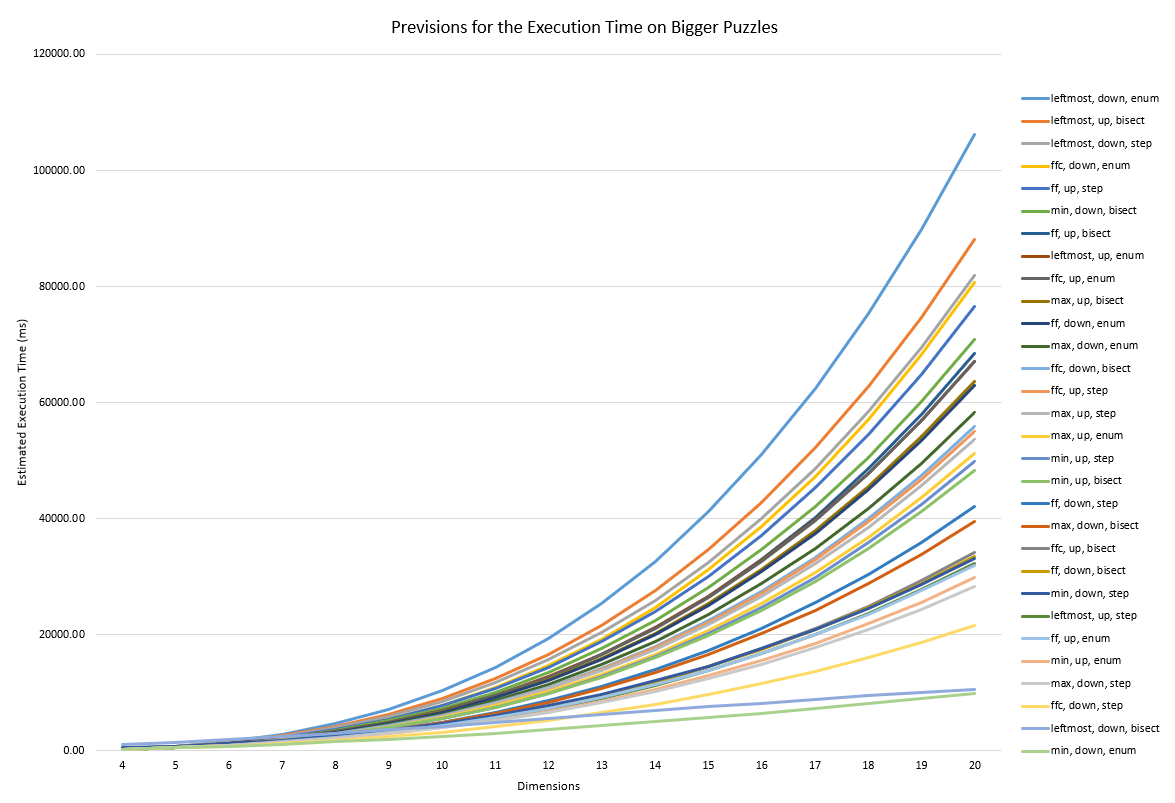
\includegraphics[width=\textwidth]{img/previsions.png}
    \caption{Execution Times Predictions} \label{fig4}
\end{figure}

\newpage

\subsection{Dimensional Analysis}

We will be using "ff, up, bisect" as a labeling option since it
    is the better one for grids up to 7x7, as already mentioned.

\begin{figure} [h]
    \centering
    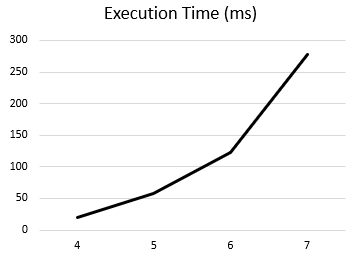
\includegraphics[scale=0.6]{img/dimensional_analysis.png}
    \caption{Execution Times} \label{fig5}
\end{figure}

As we can see in Figure \ref{fig5}, when the grid's dimension increases,
    the execution time also increases.

To know the rate at which this increase happens, we need to find an appropriate regression function.
This function will establish a relation between the grid's dimensions and the execution time.
However, with only 4 points, we can't estimate with certainty what will be the behavior
    of the best regression function.

\begin{figure} [h]
    \centering
    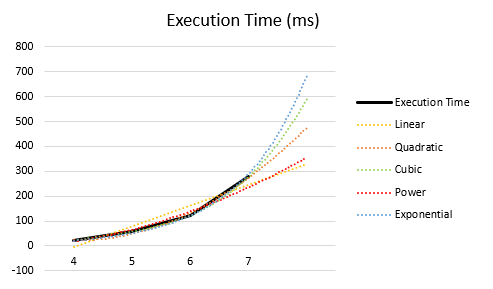
\includegraphics[scale=0.6]{img/dimensional_prediction.png}
    \caption{Execution Times With Trendlines} \label{fig6}
\end{figure}

From all the data we have, the best approximation is a cubic, a third-degree polynomial,
    as demonstrated in Figure \ref{fig6}.

\section{Conclusions and Future Work}
Upon starting this project, some assumptions where made about the ideal labelling options
for solving these types of puzzles.

Initially the idea has that either "ff" or "ffc" where the ideal forms of selecting the
next variables to explore, this would emulate the form that a human would solve these puzzles,
focussing on the variables that only have one value possible.
There was also the assumption that the type of selection of values was of little importance.
Since the domain is so small, only a total of 3 possible variables and no "greater than" or 
"less than" types of restrictions, the difference in performance of "step", "enum" or "bisect"
and of "up" or "down" would average out too negligible.

Upon analysing the results some of our assumptions seem correct. The choice between "up"
and "down" seems of little to no importance, with any increased performance of one over the
other being incidental. The results for using either "step", "enum" or "bisect" don't
demonstrate any clear pattern, being to scatter to draw any solid conclusions.

But, unlike what was assumed, when choosing the method of selecting the next variable to explore,
the results were a lot different than expected. It was expected that either "ff" or "ffc"
would be the ideal way of selecting variables, but the results where to scatter to both prove
or disprove that theory. The data shows that for 7x7 puzzles the ideal option is "ff, up, bisect",
but our predictions for greater dimensions shows that "min, down, enum" or "leftmost, down, bisect"
would be better options. One can postulate that what is happening is that is more efficient to start
with a somewhat random variable, explore the options of this variable and use the more constrained
variables as way to eliminate invalid values for the starting variable, but further and bigger tests
cases, meaning puzzles, would be necessary to test this theory.

In conclusion, although some insight can already be obtained by the tests already executed, no
solid conclusion can be reached without more puzzles, preferably ones with larger dimensions.
Still it is our belief that this is a good starting point for any further exploration of tricky
triple puzzles.

\section{References}
\begin{enumerate}
    \item Tricky Triple Puzzle Page: https://erich-friedman.github.io/puzzle/shape/
    \item SICStus Prolog Documentation: https://sicstus.sics.se/documentation.html
\end{enumerate}

\newpage
\section{Annex}

\subsection{Average Execution Times Table} \label{experiment-results}

\begin{table} [h]
    \caption{Average Times Obtained (ms)} \label{tab1}
    \begin{tabularx}{\textwidth}{|C|C|C|C|C|C|C|}
        \hline
        \multicolumn{3}{|c|}{Labeling} & \multicolumn{4}{|c|}{Grids} \\
        \cline{4-7}
        \multicolumn{3}{|c|}{Options} & 4x4 & 5x5 & 6x6 & 7x7 \\
        \hline
        leftmost & up   & step   & 13.43 & 44.57 & 131.4  & 296.75 \\
        leftmost & up   & enum   & 20.14 & 53.57 & 128    & 304.75 \\
        leftmost & up   & bisect & 13.43 & 46.86 & 131.2  & 347.75 \\
        leftmost & down & step   & 17.71 & 51.43 & 140.6  & 359.25 \\
        leftmost & down & enum   & 17.86 & 53.57 & 128.2  & 343.75 \\
        leftmost & down & bisect & 17.71 & 47    & 150    & 320.25 \\
        ff       & up   & step   & 13.42 & 60.14 & 143.8  & 336    \\
        ff       & up   & enum   & 26.71 & 46.86 & 131.2  & 301    \\
        ff       & up   & bisect & 20    & 58    & 122    & 277.25 \\
        ff       & down & step   & 18    & 49.14 & 128    & 289    \\
        ff       & down & enum   & 15.71 & 49.14 & 128    & 308.5  \\
        ff       & down & bisect & 15.71 & 44.57 & 134.4  & 308.5  \\
        ffc      & up   & step   & 11.14 & 51.43 & 134.4  & 308.5  \\
        ffc      & up   & enum   & 13.29 & 53.57 & 131.4  & 308.5  \\
        ffc      & up   & bisect & 11.14 & 44.57 & 131.4  & 296.75 \\
        ffc      & down & step   &  9.71 & 46.86 & 134.4  & 285    \\
        ffc      & down & enum   & 15.57 & 58.14 & 121.8  & 285.25 \\
        ffc      & down & bisect & 15.57 & 49    & 125    & 293    \\
        min      & up   & step   & 15.71 & 44.58 & 118.8  & 281.25 \\
        min      & up   & enum   & 15.57 & 49.14 & 137.4  & 300.75 \\
        min      & up   & bisect & 13.43 & 44.71 & 131.2  & 312.5  \\
        min      & down & step   & 17.86 & 44.57 & 131.4  & 300.5  \\
        min      & down & enum   & 15.71 & 46.86 & 143.8  & 304.5  \\
        min      & down & bisect & 13.43 & 46.86 & 125    & 312.5  \\
        max      & up   & step   & 13.43 & 44.58 & 125    & 300.75 \\
        max      & up   & enum   & 13.43 & 49    & 131.4  & 304.5  \\
        max      & up   & bisect & 13.29 & 47    & 125    & 304.5  \\
        max      & down & step   & 13.43 & 44.71 & 134.4  & 300.75 \\
        max      & down & enum   & 17.86 & 44.58 & 122    & 300.75 \\
        max      & down & bisect & 20    & 42.43 & 122    & 289    \\
        \hline
    \end{tabularx}
\end{table}

\newpage
\subsection{Trendlines using to Estimate Execution Time for Bigger Grids} \label{trendlines}
In the following equations,
\begin{itemize}
    \item \(x\) = Grid's Dimensions
    \item \(y\) = Execution Time
\end{itemize}

\begin{table} [h]
    \caption{Trendlines} \label{tab2}
    \begin{tabularx}{\textwidth}{|C|C|C|C|C|}
        \hline
        \multicolumn{3}{|c|}{Labeling Options} & \multicolumn{2}{|c|}{Equations} \\
        \hline
        leftmost & up   & step   & \multicolumn{2}{|c|}{\(y =  12.337x^3 - 46.293x^2 + 86.235x - 34.564 = 0 \)} \\
        leftmost & up   & enum   & \multicolumn{2}{|c|}{\(y =  13.549x^3 - 55.836x^2 + 106.09x - 50.379 = 0 \)} \\
        leftmost & up   & bisect & \multicolumn{2}{|c|}{\(y =  17.001x^3 -  82.55x^2 + 164.36x -  80.95 = 0 \)} \\
        leftmost & down & step   & \multicolumn{2}{|c|}{\(y =  11.933x^3 - 53.128x^2 + 122.57x - 67.943 = 0 \)} \\
        leftmost & down & enum   & \multicolumn{2}{|c|}{\(y = -1.0774x^3 + 43.321x^2 + 93.137x + 68.607 = 0 \)} \\
        leftmost & down & bisect & \multicolumn{2}{|c|}{\(y =  6.6024x^3 - 12.286x^2 + 21.112x - 2.2714 = 0 \)} \\
        ff       & up   & step   & \multicolumn{2}{|c|}{\(y =  10.774x^3 - 42.286x^2 + 84.869x - 39.929 = 0 \)} \\
        ff       & up   & enum   & \multicolumn{2}{|c|}{\(y =   9.369x^3 -   33.5x^2 + 68.345x -   28.5 = 0 \)} \\
        ff       & up   & bisect & \multicolumn{2}{|c|}{\(y =  3.8833x^3 + 7.1857x^2 - 19.883x + 24.529 = 0 \)} \\
        ff       & down & step   & \multicolumn{2}{|c|}{\(y =  8.0738x^3 -   27.1x^2 + 65.069x -   34.9 = 0 \)} \\
        ff       & down & enum   & \multicolumn{2}{|c|}{\(y =  10.288x^3 - 42.957x^2 +  97.14x - 51.186 = 0 \)} \\
        ff       & down & bisect & \multicolumn{2}{|c|}{\(y =   10.22x^3 - 40.821x^2 + 84.351x - 33.607 = 0 \)} \\
        ffc      & up   & step   & \multicolumn{2}{|c|}{\(y = -0.3405x^3 + 34.943x^2 - 71.302x + 52.414 = 0 \)} \\
        ffc      & up   & enum   & \multicolumn{2}{|c|}{\(y =  7.3119x^3 - 20.457x^2 +  45.76x - 19.186 = 0 \)} \\
        ffc      & up   & bisect & \multicolumn{2}{|c|}{\(y =  9.5357x^3 - 35.071x^2 + 72.179x - 33.357 = 0 \)} \\
        ffc      & down & step   & \multicolumn{2}{|c|}{\(y =  3.5429x^3 + 10.843x^2 - 37.186x + 49.514 = 0 \)} \\
        ffc      & down & enum   & \multicolumn{2}{|c|}{\(y =  3.4012x^3 + 6.9357x^2 - 11.044x + 16.279 = 0 \)} \\
        ffc      & down & bisect & \multicolumn{2}{|c|}{\(y =  7.6726x^3 - 21.393x^2 + 41.613x - 14.464 = 0 \)} \\
        min      & up   & step   & \multicolumn{2}{|c|}{\(y =   3.044x^3 + 10.936x^2 -  22.83x + 22.279 = 0 \)} \\
        min      & up   & enum   & \multicolumn{2}{|c|}{\(y =  8.4345x^3 -  25.25x^2 + 43.423x -   8.75 = 0 \)} \\
        min      & up   & bisect & \multicolumn{2}{|c|}{\(y =  3.6929x^3 +    7.9x^2 + 22.836x +   29.1 = 0 \)} \\
        min      & down & step   & \multicolumn{2}{|c|}{\(y =   3.806x^3 + 5.0071x^2 -  10.52x + 15.136 = 0 \)} \\
        min      & down & enum   & \multicolumn{2}{|c|}{\(y =  4.1869x^3 + 1.5786x^2 - 0.6155x + 5.9929 = 0 \)} \\
        min      & down & bisect & \multicolumn{2}{|c|}{\(y =  8.2381x^3 - 28.143x^2 +  60.19x + 24.714 = 0 \)} \\
        max      & up   & step   & \multicolumn{2}{|c|}{\(y =  5.7381x^3 - 10.571x^2 +  22.69x + 0.1429 = 0 \)} \\
        max      & up   & enum   & \multicolumn{2}{|c|}{\(y =  5.0476x^3 - 1.7143x^2 - 7.7619x + 24.429 = 0 \)} \\
        max      & up   & bisect & \multicolumn{2}{|c|}{\(y =  13.118x^3 - 68.164x^2 + 155.24x - 84.621 = 0 \)} \\
        max      & down & step   & \multicolumn{2}{|c|}{\(y =  2.1095x^3 + 12.543x^2 - 15.252x + 10.314 = 0 \)} \\
        max      & down & enum   & \multicolumn{2}{|c|}{\(y =  7.1417x^3 - 20.164x^2 + 39.358x - 10.621 = 0 \)} \\
        max      & down & bisect & \multicolumn{2}{|c|}{\(y =  10.875x^3 -  52.25x^2 + 118.62x -  57.25 = 0 \)} \\
        \hline
    \end{tabularx}
\end{table}

\end{document}
